\chapter{Introducción}




% \begin{tblr}{|Q[h,t]|Q[c,t]|Q[r,b]|}
% \hline
% {C[Au].c1ccc(cc1)P(c2ccccc2)c3ccccc3 \\ Left Left} & Middle Center & {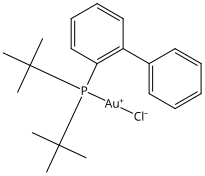
\includegraphics{imagenes/SciFinder/Chloro[(1,1-biphenyl-2-yl)di-tert-butylphosphine]gold(I).png}} \\
% \hline
% \end{tblr}

\textbf{Meter aqui una introduccion general sobre la química, la quimica informatica (y cómo surge en base a las necesidades computacionales), mencionar brevemente la organometalica (mas tarde en la seccion de estado del arte profundizo, junto con cosas de dibujado, tutorial de SMILES, y representacion de moléculas)}


\section{Motivación y objetivos}

Los formatos de notación lineal llevan siendo un tema de interés e investigación para los científicos desde mediados del siglo 19 \cite{107_years_linear_notations} \textbf{Terminar esto}

En la actualidad, existen varias representaciones lineales \textbf{(Para esto debo haber hablado antes de las representaciones lineales, o bien lo explico aquí, o bien lo redirijo a los fundamentos teóricos. O bien, justo antes de empezar este párrafo, que será lo mejor-> quitar entonces la siguiente negrita)}, siendo las más usadas SMILES, InChI, y SELFIES \cite{SELFIES}. \textbf{Como comenté antes, una forma muy potente de representar moléculas y compuestos químicos es mediante cadenas strings}, y de esto justamente se encargan las representaciones lineales: traducir una molécula, con sus átomos, enlaces entre ellos, ciclos y otras propiedades características, en una cadena string que la represente, y que la máquina y los propios químicos puedan entender. Sin embargo, hay diferencias notables entre las representaciones, tanto en la sintaxis de las cadenas que se generan como en las aplicaciones que se le puede dar a cada una de ellas.

SMILES, ideada por David Weininger, sale a la luz en 1988 satisfaciendo con creces las necesidades de procesamiento de información química que había, desbancando a la representación estandarizada del momento, Wiswesser Line Notation (WLN). Desde ese entonces SMILES se convirtió —y sigue siendo a día de hoy— en el estándar de representación lineal, ya que permite describir estructuras moleculares de una forma sencilla en un formato fácil de leer, lo que ha hecho que sea una herramienta popular en la química computacional, siendo la más usada entre investigadores y químicos. Pese a esto, SMILES tiene dos grandes inconvenientes: una misma molécula puede escribirse con varias cadenas SMILES distintas válidas, es decir, tiene sinónimos (Figura \ref{fig:sinonimos_smiles}); y no es robusto ni sintáctica ni semánticamente. En este sentido se podría generar un string que no represente una molécula válida, como lo es \emph{CC(CCCC}, el cual tiene un paréntesis sin cerrar (lo que implica que no se delimita cuándo acaba la rama). O generar una molécula que no sea químicamente viable como \emph{CO=CC}, que muestra un átomo de oxígeno neutro formando tres enlaces (superando el límite de enlaces covalentes que un oxígeno neutro puede tener) \cite{SELFIES}.

\begin{figure}[H]
\centering
    \fbox{
\includegraphics[scale=0.3]{imagenes/placeholder.png}}  
    \caption{Distintas cadenas SMILES válidas para la misma molécula de <nombre-molecula>. \cite{}}
    \label{fig:sinonimos_smiles}
\end{figure}

Esto tiene especial relevancia en el ámbito del Machine Learning (ML). Aunque se sale del alcance de este trabajo, uno de los grandes objetivos de la química computacional es la creación o diseño de nuevas moléculas. Se podrían crear modelos de ML o redes neuronales capaces de generar moléculas ficticias válidas, para posteriormente ver sus propiedades, valorarlas energéticamente para ver cuán estables son, y estudiar su viabilidad en distintas aplicaciones, entre otras cosas. SMILES dificulta esta tarea, y por ello, aparece en 2020, SELFIES (SELF-referencIng Embedded Strings), una nueva representación lineal 100\% robusta, muy usada actualmente para modelos generativos. Ver \cite{SELFIES, krenn_self_referencing_2020} para más detalles de cómo soluciona los problemas de robustez y otras características de la representación. SELFIES es relativamente reciente y continuamente está ampliando sus funcionalidades, mejorando su simplicidad y facilidad de uso para el usuario \cite{selfies_recent_2023}. Aun así, no se termina de instaurar entre la comunidad investigadora. 

\textbf{AQUI METER ALGO DE InChI, o lo meto arriba, antes de hablar sobre SELFIES.
}

Por todo lo anterior, me centraré en la notación SMILES durante el desarrollo de este trabajo. Dicho esto, existen diversas fuentes de datos en química donde se recoge gran cantidad de información acerca de los compuestos. Menciono las más importantes y las que serán objeto de interés. \emph{PubChem}, una base de datos abierta que sirve información a millones de usuarios en todo el mundo, desde investigadores y estudiantes hasta el público general. Recogen para cada compuesto, información sobre su estructura, representaciones 2D y 3D, identificadores, propiedades químicas y físicas, patentes, avisos de toxicidad, etc. \cite{pubchem_website} 

\emph{SciFinder}, una herramienta de investigación muy potente que permite explorar las bases de datos de CAS (American Chemical Society) las cuales contienen literatura sobre Química y otras disciplinas afines como Física, Biomedicina, Geología, Ingeniería Química, etc. Incluye referencias bibliográficas y resúmenes de artículos, informes, y libros entre otras cosas. Permite realizar búsquedas por estructura, nombres de sustancias o identificadores, reacciones en la que participa dicha sustancia, artículos y publicaciones que nombren el compuesto en cuestión, e incluso proveedores de compra. Para el uso de esta herramienta es necesario acceder mediante la red de una institución autorizada (en este caso trabajo mediante VPN de la UGR) y seguir los pasos para registrarte \footnote{Pasos para el registro en SciFinder \url{https://bibliotecaugr.libguides.com/scifinder_scholar}}

uno de los principales problemas que se detectan es la heterogeneidad en las distintas bases de datos \textbf{continuar esto}



\textbf{Aquí empezar ya con la tabla comparativa. Para eso, tengo que introducir las fuentes de datos }

\noindent \textbf{Meter parrafo de los quimicos colaboradores...mirar pedro}

Por todo lo anterior, una solución que permita aunar... \textbf{continuar esto}  

Por tanto, el objetivo principal de este Trabajo Fin de Grado sería modificar el paquete OpenBabel creando un método para canonizar códigos SMILES, orientado específicamente para compuestos organometálicos, de los cuales dispongo de un conjunto de datos de 30 moléculas considerados de interés por la tutora y los químicos con los que colabora. Para ello, se establecen los siguientes subobjetivos:
\begin{itemize}
    \item Analizar y comparar las cadenas SMILES de distintas bases de datos (p.ej. Sigma-Aldrich, SciFinder) viendo los posibles sinónimos para una misma molécula.
    \item Determinar un sistema que genere, a partir de cualquier sinónimo SMILES de la misma molécula, un único SMILES canónico.
    \item Definir otro algoritmo o conjunto de reglas que mejore, aunque sea mínimamente, el sistema de dibujado de los compuestos.
\end{itemize} 



\begin{table}
\small
  \begin{tabular}
      {lc} \hline Código SMILES & Representación 2D \\ \hline C[Au].c1ccc(cc1)P(c2ccccc2)c3ccccc3 & \parbox[c]{5em}{
      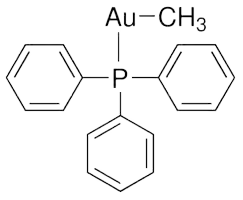
\includegraphics[width=2cm]{imagenes/SigmaAldrich/Methyl(triphenylphosphine)gold(I).png}} \\ \hline
      Cl[Pd]Cl.C1CC=CCCC=C1 & \parbox[r]{5em}{
      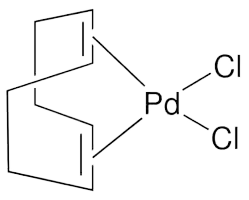
\includegraphics[width=2cm]{imagenes/SigmaAldrich/Dichloro(1,5-cyclooctadiene)palladium(II).png}} \\ \hline
      Cl[Au].CP(C)C & \parbox[c]{5em}{
      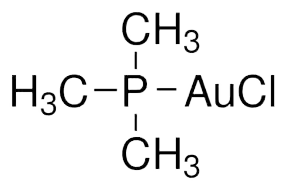
\includegraphics[width=2cm]{imagenes/SigmaAldrich/Chloro(trimethylphosphine)gold(I).png}} \\ \hline
      Cl[Au].CC(C)(C)P(c1ccccc1-c2ccccc2)C(C)(C)C & \parbox[c]{5em}{
      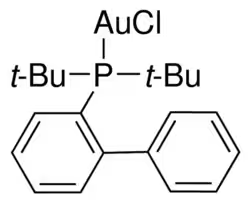
\includegraphics[width=2cm]{imagenes/SigmaAldrich/Chloro[(1,1-biphenyl-2-yl)di-tert-butylphosphine]gold(I).png}} \\ \hline
      [Fe]I.[C-]\#[O+].[C-]\#[O+].[CH]1[CH][CH][CH][CH]1 & \parbox[c]{5em}{
      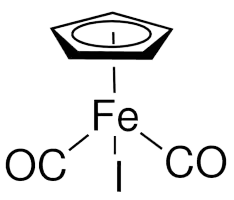
\includegraphics[width=2cm]{imagenes/SigmaAldrich/Dicarbonylcyclopentadienyliodoiron(II).png}} \\ \hline
  \end{tabular}
  \caption{Códigos SMILES y sus representaciones 2D según Sigma-Aldrich}
\end{table}


\begin{table}
\small
  \begin{tabular}
      {lc} \hline Código SMILES & Representación 2D \\ \hline 
      [Au+]([CH3-])[P](C=1C=CC=CC1)(C=2C=CC=CC2)C=3C=CC=CC3 & \parbox[c]{5em}{
      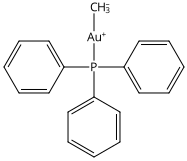
\includegraphics[width=2cm]{imagenes/SciFinder/Methyl(triphenylphosphine)gold(I).png}} \\ \hline
      [Cl-][Pd+2]123([Cl-])[CH]=4CC[CH]3=[CH]2CC[CH]41 & \parbox[r]{5em}{
      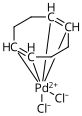
\includegraphics[width=2cm]{imagenes/SciFinder/Dichloro(1,5-cyclooctadiene)palladium(II).png}} \\ \hline
      [Cl-][Au+][P](C)(C)C & \parbox[c]{5em}{
      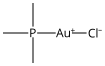
\includegraphics[width=2cm]{imagenes/SciFinder/Chloro(trimethylphosphine)gold(I).png}} \\ \hline
      [Cl-][Au+][P](C=1C=CC=CC1C=2C=CC=CC2)(C(C)(C)C)C(C)(C)C & \parbox[c]{5em}{
      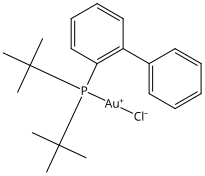
\includegraphics[width=2cm]{imagenes/SciFinder/Chloro[(1,1-biphenyl-2-yl)di-tert-butylphosphine]gold(I).png}} \\ \hline
      O\#C[Fe+2]1234([I-])(C\#O)[CH]=5[CH]4=[CH]3[CH-]2[CH]51 & \parbox[c]{5em}{
      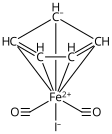
\includegraphics[width=2cm]{imagenes/SciFinder/Dicarbonylcyclopentadienyliodoiron(II).png}} \\ \hline
  \end{tabular}
  \caption{Códigos SMILES y sus representaciones 2D según SciFinder}
\end{table}








\begin{table}
  \begin{tblr}
      {Q[c,t]Q[c,m]} \hline Código SMILES & Representación 2D \\ \hline 
      C[Au].c1ccc(cc1)P(c2ccccc2)c3ccccc3 & 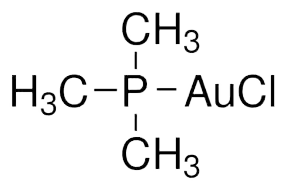
\includegraphics[width=2cm]{imagenes/SigmaAldrich/Chloro(trimethylphosphine)gold(I).png}
       \\
      Cl[Pd]Cl.C1CC=CCCC=C1 & 
      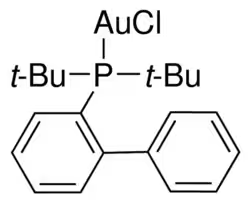
\includegraphics[width=2cm]{imagenes/SigmaAldrich/Chloro[(1,1-biphenyl-2-yl)di-tert-butylphosphine]gold(I).png} \\
      Cl[Au].CP(C)C & 
      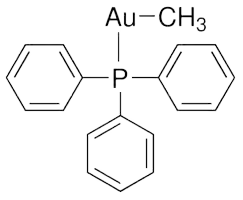
\includegraphics[width=2cm]{imagenes/SigmaAldrich/Methyl(triphenylphosphine)gold(I).png} \\
      Cl[Au].CC(C)(C)P(c1ccccc1-c2ccccc2)C(C)(C)C & 
      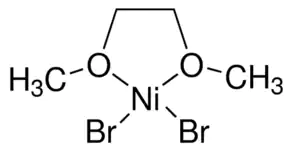
\includegraphics[width=2cm]{imagenes/SigmaAldrich/Nickel(II) bromide ethylene glycol dimethyl ether complex.png} \\ [0cm]
    [Fe]I.[C-]\#[O+].[C-]\#[O+].[CH]1[CH][CH][CH][CH]1 & 
      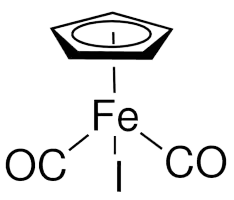
\includegraphics[width=2cm]{imagenes/SigmaAldrich/Dicarbonylcyclopentadienyliodoiron(II).png} \\ \hline
  \end{tblr}
  \caption{Códigos SMILES y sus representaciones 2D según Sigma-Aldrich}
\end{table}


% \begin{longtblr}{
%   colspec={Q[valign=t]Q[valign=b]Q[valign=h]},
%   row{1}={halign=c},
%   hlines
% }
% Id & Name & Figure \\
% 1 & Press imaginary a button & 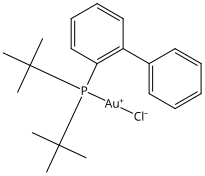
\includegraphics{imagenes/SciFinder/Chloro[(1,1-biphenyl-2-yl)di-tert-butylphosphine]gold(I).png}\\ 
% 1 & Press imaginary a button & 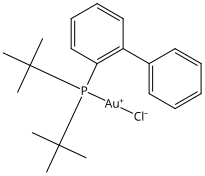
\includegraphics{imagenes/SciFinder/Chloro[(1,1-biphenyl-2-yl)di-tert-butylphosphine]gold(I).png}\\
% 1 & Press imaginary a button & 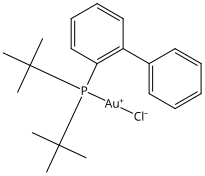
\includegraphics{imagenes/SciFinder/Chloro[(1,1-biphenyl-2-yl)di-tert-butylphosphine]gold(I).png}\\
% 1 & Press imaginary a button & 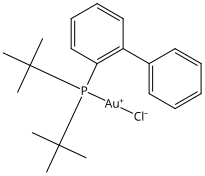
\includegraphics{imagenes/SciFinder/Chloro[(1,1-biphenyl-2-yl)di-tert-butylphosphine]gold(I).png}\\
% 1 & Press imaginary a button & 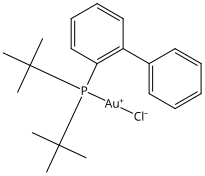
\includegraphics{imagenes/SciFinder/Chloro[(1,1-biphenyl-2-yl)di-tert-butylphosphine]gold(I).png}\\
% 1 & Press imaginary a button & 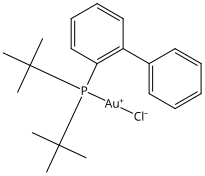
\includegraphics{imagenes/SciFinder/Chloro[(1,1-biphenyl-2-yl)di-tert-butylphosphine]gold(I).png}\\
% \end{longtblr}

\section{Objetivos}


\section{Estructura de la memoria}

% \begin{table}[ht]
%     \centering
%     \begin{tabular}{p{0.35\linewidth} | p{0.6\linewidth}}
%       Column 1  & Column2 \\ \hline
%       This text will be wrapped & Some more text \\
%       Some text here & This text maybe wrapped here if its tooooo long \\
%     \end{tabular}
%     \caption{Caption}
%     \label{tab:my_label}
% \end{table}
